% Source: ../ch01/scan.pdf pages 3 (from "Chapter 2") and 4, then scan.pdf pages 1-3
% and the top of page 4. The "9/23 Class" part of page 4 is in
% ../../Lectures/2026-09-23/notes.tex.
\documentclass[11pt]{article}
\usepackage[margin=1in]{geometry}
\usepackage{parskip}
\usepackage{amsmath,amssymb}
\usepackage{booktabs}
\usepackage{graphicx}
\usepackage{xcolor}
\usepackage{tikz}
\usepackage{pgfplots}
\pgfplotsset{compat=1.18}
\usepgfplotslibrary{groupplots}
\usepackage[hidelinks]{hyperref}

% Uncertain reading from the scan. Prints red until you fix it against the paper.
\newcommand{\unclear}[1]{\textcolor{red}{[#1?]}}

% Explanation added during processing, not written on the page.
\newenvironment{aside}{\begin{quote}\small\color{black!65}\textbf{Note.}\ }{\end{quote}}

% Shared look for the small sketches.
\pgfplotsset{sketch/.style={axis lines=none, width=5.2cm, height=4cm,
    samples=60, clip=false}}

\title{ISE 555 Reading Notes\\\large Chapter 2: Convex and Concave Functions}
\author{Luke Pepin}
\date{September 21--23, 2026}

\begin{document}
\maketitle

\section{Why Convexity Matters}

Convex and concave functions have properties that can be used to develop suitable
optimality conditions and computational schemes for optimization problems.

\section{Convex and Concave Functions}

Let $f\colon S \subseteq \mathbb{R}^n \to \mathbb{R}$, where $S$ is a non-empty
convex set.
\begin{itemize}
    \item $f$ is \textbf{convex} if its graph lies at or below every chord
          connecting two of its points.
    \item $f$ is \textbf{concave} if its graph lies at or above every chord.
\end{itemize}

\begin{center}
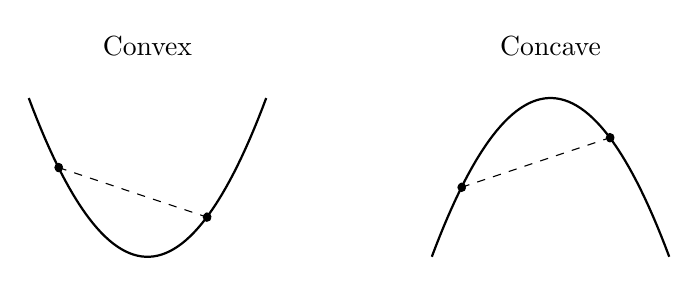
\begin{tikzpicture}
\begin{axis}[sketch, name=cvx, title={Convex}, domain=-2:2]
    \addplot[thick] {x^2};
    \addplot[dashed, mark=*, mark size=1.5pt] coordinates {(-1.5,2.25) (1,1)};
\end{axis}
\begin{axis}[sketch, at={(cvx.east)}, anchor=west, xshift=1.5cm,
             title={Concave}, domain=-2:2]
    \addplot[thick] {-x^2};
    \addplot[dashed, mark=*, mark size=1.5pt] coordinates {(-1.5,-2.25) (1,-1)};
\end{axis}
\end{tikzpicture}
\end{center}

A straight segment connecting two points of the graph is a \textbf{chord}. The
relationship must hold for \emph{every} pair of points in the domain being studied.

The expression
\[
    \lambda x_1 + (1-\lambda) x_2
\]
is a \textbf{weighted average} of two inputs $x_1$ and $x_2$. With
$0 \le \lambda \le 1$ it selects an input between them: $\lambda = 0$ or $1$ gives
an endpoint, and $\lambda = 0.5$ selects the midpoint.

\section{The Central Inequality}

\[
    \underbrace{f\big(\lambda x_1 + (1-\lambda) x_2\big)}_{\text{height of curve}}
    \;\le\;
    \underbrace{\lambda f(x_1) + (1-\lambda) f(x_2)}_{\text{height of chord}}
\]

\begin{itemize}
    \item \textbf{Left side (curve):} mix the inputs, then apply the function.
    \item \textbf{Right side (chord, the dashed line):} compute the endpoint
          outputs, then mix them.
\end{itemize}

Convexity compares these two operations.
% CHANGED: page had "less than" for convex and "<=" for concave.
% Convex is <= (at most); concave reverses the inequality to >=.
For a convex function, the first result (apply to the averaged input) is
\emph{at most} the second (average the outputs). For a concave function it is
\emph{at least} the second.

\subsection*{Example: $f(x) = x^2$ with $x_1 = 0$, $x_2 = 4$, $\lambda = 0.5$}

\begin{minipage}[c]{0.5\linewidth}
\begin{itemize}
    \item \textbf{Curve:} the halfway input is 2; squaring it gives 4.
    \item \textbf{Chord:} the endpoint outputs are 0 and $16 = 4^2$; their
          average is 8.
\end{itemize}
\centering
\begin{tabular}{lc}
    \toprule
    Input & 2 \\
    Curve & 4 \\
    Chord & 8 \\
    \bottomrule
\end{tabular}
\end{minipage}\hfill
\begin{minipage}[c]{0.45\linewidth}
\centering
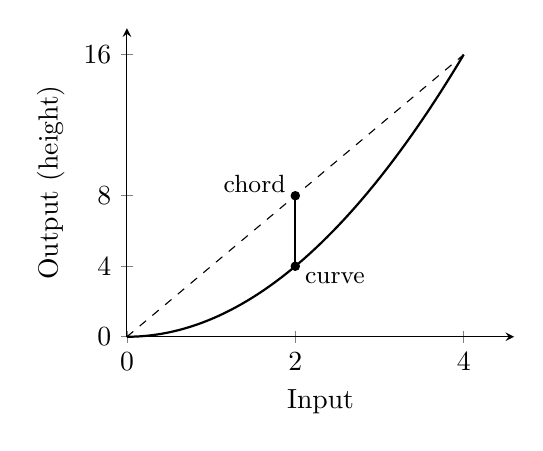
\begin{tikzpicture}
\begin{axis}[width=6.5cm, height=5.5cm, axis lines=left,
             xlabel={Input}, ylabel={Output (height)},
             xmin=0, xmax=4.6, ymin=0, ymax=17.5,
             xtick={0,2,4}, ytick={0,4,8,16}, clip=false]
    \addplot[thick, domain=0:4, samples=60] {x^2};
    \addplot[dashed] coordinates {(0,0) (4,16)};
    \draw[thick] (axis cs:2,4) -- (axis cs:2,8);
    \addplot[only marks, mark=*, mark size=1.5pt] coordinates {(2,4) (2,8)};
    \node[right, font=\small] at (axis cs:2,3.3) {curve};
    \node[left, font=\small] at (axis cs:2,8.7) {chord};
\end{axis}
\end{tikzpicture}
\end{minipage}

\section{Convex Sets}

\begin{itemize}
    \item A \textbf{set} is a collection of allowed inputs.
    \item A set is \textbf{convex} if the entire straight segment between any two
          of its points is allowed, so the set has no gaps.
    \item The \textbf{domain} is the set of allowed inputs.
\end{itemize}

Keep the two ideas separate:
\begin{itemize}
    \item A \emph{convex set} describes which inputs are allowed.
    \item A \emph{convex or concave function} describes the relationship between
          a graph and its chords.
\end{itemize}

\section{Derivative Tests}

\begin{itemize}
    \item $f(x)$ is the graph's height.
    \item $f'(x)$, the first derivative, is the slope: positive means rising, zero
          means flat, negative means falling.
\end{itemize}

\begin{itemize}
    \item \textbf{Convex:} the slope never decreases as $x$ increases (the function
          falls more slowly, or rises faster).
    \item \textbf{Concave:} the slope never increases as $x$ increases (the
          function rises more slowly).
\end{itemize}

Convexity describes how the slope \emph{changes}, not whether the function itself
rises or falls.

\begin{center}
\begin{tabular}{lll}
    \toprule
    Throughout the interval & Meaning & Classification \\
    \midrule
    $f''(x) \ge 0$ & slope never decreases & convex \\
    $f''(x) \le 0$ & slope never increases & concave \\
    \bottomrule
\end{tabular}
\end{center}

For example, $f(x) = x^2 \Rightarrow f'(x) = 2x \Rightarrow f''(x) = 2$, so $f$ is
convex. Check the whole interval: one point does not establish convexity over the
whole domain.

\subsection*{Example: classify $f(x) = x^2 - 4x + 3$ over all real numbers}

\[
    f'(x) = 2x - 4, \qquad f''(x) = 2 \ge 0,
\]
so $f$ is \textbf{convex}. Any chord lies higher than the curve between its
endpoints.

\begin{center}
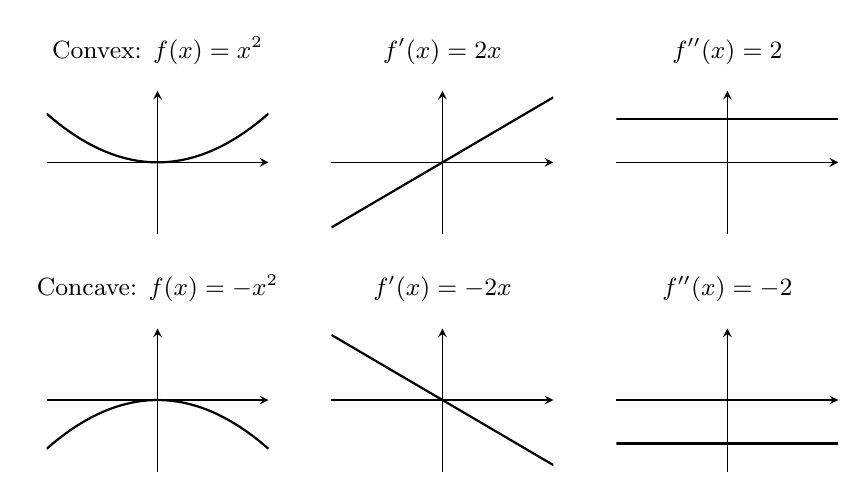
\begin{tikzpicture}
\begin{groupplot}[group style={group size=3 by 2, horizontal sep=0.8cm,
                              vertical sep=1.2cm},
                  width=4.4cm, height=3.4cm, axis lines=middle,
                  xtick=\empty, ytick=\empty, domain=-1.5:1.5, samples=40,
                  ymin=-3.3, ymax=3.3, title style={font=\small}]
    \nextgroupplot[title={Convex: $f(x) = x^2$}]
        \addplot[thick] {x^2};
    \nextgroupplot[title={$f'(x) = 2x$}]
        \addplot[thick] {2*x};
    \nextgroupplot[title={$f''(x) = 2$}]
        \addplot[thick] {2};
    \nextgroupplot[title={Concave: $f(x) = -x^2$}]
        \addplot[thick] {-x^2};
    \nextgroupplot[title={$f'(x) = -2x$}]
        \addplot[thick] {-2*x};
    \nextgroupplot[title={$f''(x) = -2$}]
        \addplot[thick] {-2};
\end{groupplot}
\end{tikzpicture}
\end{center}

For the convex function the slope $f'$ is always increasing ($f'' > 0$); for the
concave function it is always decreasing ($f'' < 0$). At \textbf{inflection
points}, concavity changes.

\section{Strict Convexity}

% CHANGED: page had "requires chord to stay strictly below curve". It is the curve
% that stays strictly below the chord (page 3 of the same scan says so correctly),
% and the two meet at the chord's endpoints, so "strictly" applies between them.
A function is \textbf{strictly convex} if the curve stays strictly below every chord
between the chord's endpoints. The chord height can never equal the actual curve
height there. A strictly convex function can have at most one minimum point.

\begin{center}
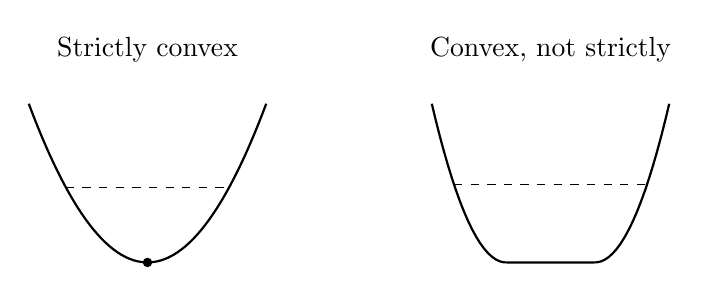
\begin{tikzpicture}
\begin{axis}[sketch, name=strict, title={Strictly convex}, domain=-1.6:1.6]
    \addplot[thick] {x^2};
    \addplot[dashed] coordinates {(-1.1,1.21) (1.1,1.21)};
    \addplot[only marks, mark=*, mark size=1.5pt] coordinates {(0,0)};
\end{axis}
\begin{axis}[sketch, at={(strict.east)}, anchor=west, xshift=1.5cm,
             title={Convex, not strictly}, domain=-1.6:1.6]
    \addplot[thick] {(abs(x)>0.6)*1.8*(abs(x)-0.6)^2};
    \addplot[dashed] coordinates {(-1.3,0.882) (1.3,0.882)};
\end{axis}
\end{tikzpicture}
\end{center}

The flat bottom on the right is where a chord can lie on the curve itself, and
every point along it is a minimum.

\section{Sublevel and Superlevel Sets}

The \textbf{sublevel set} of $f$ at height $a$ is
\[
    A_a = \{\, x : f(x) \le a \,\},
\]
all inputs whose output is at most $a$.

\subsection*{Example: $f(x) = x^2$ with height limit 4}

\[
    A_4 = \{\, x : x^2 \le 4 \,\} = [-2, 2].
\]
Picture a horizontal line at height 4, then collect the inputs where the curve is
at or below it. Those inputs form an interval with no gaps, which is a convex set.

\textbf{Every sublevel set of a convex function is convex.}

If a cost function is convex, blending two affordable choices stays affordable.
With a budget of 100 and $f(x_1), f(x_2) \le 100$:
\[
    f\big(\lambda x_1 + (1-\lambda) x_2\big) \le \lambda f(x_1) + (1-\lambda) f(x_2) \le 100,
\]
that is, blended choice $\le$ blended endpoint cost $\le$ budget.

For a \textbf{concave} function the matching idea uses the \textbf{superlevel set}
$\{\, x : f(x) \ge a \,\}$. With two plans that each earn at least \$100, the profit
of a blend is at least the average of the endpoint profits, which is at least 100.

Convex sublevel sets do \emph{not} prove that the function itself is convex.

\begin{aside}
For example, $f(x) = \sqrt{|x|}$ has convex sublevel sets
$\{x : \sqrt{|x|} \le a\} = [-a^2, a^2]$, but $f$ is not convex: the chord from
$x = 0$ to $x = 1$ lies below the curve.
\end{aside}

\section{Composition and the Chain Rule}

Let $h(x) = g(f(x))$. If $g$ is convex and \textbf{non-decreasing} (larger inputs
never cause smaller values) and $f$ is convex, then $h$ is convex.

Chain rule:
\[
    h'(x) = g'(f(x))\, f'(x).
\]
Examples:
\begin{align*}
    (3x+1)^2 &\;\to\; 2(3x+1) \cdot 3 = 6(3x+1), \\
    (2x+5)^2 &\;\to\; 2(2x+5) \cdot 2 = 4(2x+5) = 8x + 20.
\end{align*}

\section{Tangent Lines}

The tangent line to $f$ at $x = a$ is
\[
    T(x) = f(a) + f'(a)(x - a).
\]
For example, with $f(x) = x^2$ and $a = 1$,
\[
    T(x) = 1 + 2(x - 1) = 2x - 1.
\]
At $x = 2$ the tangent predicts a height of 3, while the curve's actual height is 4.

\begin{center}
\begin{tabular}{lll}
    \toprule
    The curve is\ldots & relative to a chord & relative to a tangent \\
    \midrule
    Convex  & below (chord overestimates) & above (tangent underestimates) \\
    Concave & above & below \\
    \bottomrule
\end{tabular}
\end{center}

\begin{center}
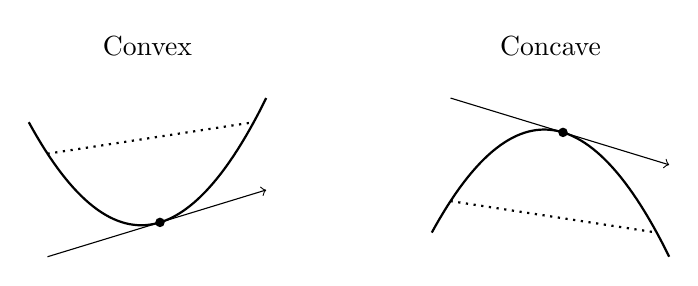
\begin{tikzpicture}
\begin{axis}[sketch, name=ct1, title={Convex}, domain=-1.8:2]
    \addplot[thick] {x^2};
    \addplot[dotted, thick] coordinates {(-1.5,2.25) (1.8,3.24)};
    \addplot[->, domain=-1.5:2] {0.6*x - 0.09};
    \addplot[only marks, mark=*, mark size=1.5pt] coordinates {(0.3,0.09)};
\end{axis}
\begin{axis}[sketch, at={(ct1.east)}, anchor=west, xshift=1.5cm,
             title={Concave}, domain=-1.8:2]
    \addplot[thick] {-x^2};
    \addplot[dotted, thick] coordinates {(-1.5,-2.25) (1.8,-3.24)};
    \addplot[->, domain=-1.5:2] {-0.6*x + 0.09};
    \addplot[only marks, mark=*, mark size=1.5pt] coordinates {(0.3,-0.09)};
\end{axis}
\end{tikzpicture}
\end{center}

If the slope at $a$ is zero, $f'(a) = 0$, then the inequality becomes
\[
    f(x) \ge f(a).
\]
Every other value is at least as high as $f(a)$, so $a$ is a \textbf{global
minimum} (if $f$ is convex).

\begin{aside}
``The inequality'' is the tangent-line inequality for a differentiable convex
function, $f(x) \ge f(a) + f'(a)(x - a)$ for all $x$: the curve lies above every
tangent. Setting $f'(a) = 0$ gives $f(x) \ge f(a)$.
\end{aside}

\end{document}
